\documentclass[tikz,border=5pt,multi=tikzpicture]{standalone}
\usepackage[UTF8]{ctex}
\usepackage{amsmath}
\usetikzlibrary{arrows.meta,calc}
\definecolor{ink}{HTML}{17365D}
\definecolor{field}{HTML}{287DA8}
\definecolor{force}{HTML}{C56B2A}
\definecolor{inner}{HTML}{5E823F}
\tikzset{every node/.style={font=\small},vec/.style={-{Stealth[length=2mm]},thick},helper/.style={gray,dashed}}
\begin{document}
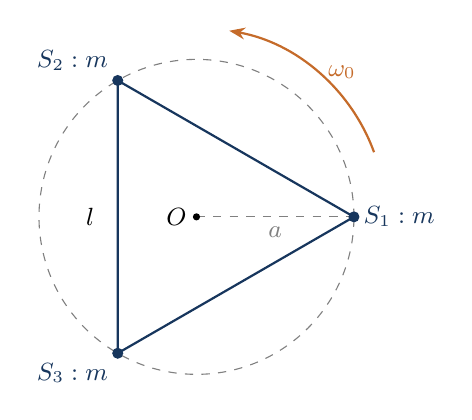
\begin{tikzpicture}
  \foreach \j/\angle in {1/0,2/120,3/240}{\coordinate (S\j) at (\angle:2);}
  \draw[helper] (0,0) circle (2);
  \draw[thick,ink] (S1)--(S2)--(S3)--cycle;
  \draw[helper] (0,0)--(S1) node[midway,below] {$a$};
  \fill (0,0) circle (1.3pt) node[left] {$O$};
  \fill[ink] (S1) circle (2pt) node[right] {$S_1:m$};
  \fill[ink] (S2) circle (2pt) node[above left] {$S_2:m$};
  \fill[ink] (S3) circle (2pt) node[below left] {$S_3:m$};
  \node[left,xshift=-5pt] at ($(S2)!.5!(S3)$) {$l$};
  \draw[vec,force] (20:2.4) arc (20:80:2.4) node[midway,right] {$\omega_0$};
\end{tikzpicture}
\begin{tikzpicture}
  \coordinate (O) at (0,0);
  \coordinate (S1) at (2,0);\coordinate (S2) at (120:2);\coordinate (S3) at (240:2);
  \draw[helper] (S1)--(S2)--(S3)--cycle;
  \draw[helper] (O)--(S1);
  \fill (O) circle (1.3pt) node[below] {$O$};
  \fill[ink] (S1) circle (2pt) node[right] {$S_1$};
  \fill[ink] (S2) circle (2pt) node[above left] {$S_2$};
  \fill[ink] (S3) circle (2pt) node[below left] {$S_3$};
  \draw[vec,field] (S1)--++(150:1.0) node[above] {$\boldsymbol F_{12}$};
  \draw[vec,field] (S1)--++(210:1.0) node[below] {$\boldsymbol F_{13}$};
  \draw[vec,force,line width=1.2pt] (S1)--++(180:1.73205) node[midway,above] {$\boldsymbol F$};
  \node[align=left,anchor=west] at (3.1,.8) {$F_{12}=F_{13}=Gm^2/l^2$\\[4pt]两力夹角 $60^\circ$\\[4pt]合力指向共同质心 $O$};
\end{tikzpicture}
\begin{tikzpicture}[scale=1.9]
  \foreach \j/\angle in {1/0,2/120,3/240}{
    \coordinate (S\j) at (\angle:1);
    \draw[helper] (0,0)--(\angle:2.15);
    \draw[helper] (0,0)--({\angle+180}:1.72);
  }
  \draw[thin,ink] (S1)--(S2)--(S3)--cycle;
  \fill (0,0) circle (.025) node[below left] {$O$};
  \foreach \j/\angle in {1/0,2/120,3/240}{
    \fill[ink] (\angle:1) circle (.03);
  }
  \node[right] at (S1) {$S_1$};\node[above left] at (S2) {$S_2$};\node[below left] at (S3) {$S_3$};
  \foreach \j/\angle in {1/0,2/120,3/240}{
    \fill[force] (\angle:2.04381719) circle (.028);
    \fill[inner] ({\angle+180}:.41388793) circle (.028);
    \fill[field] ({\angle+180}:1.61978961) circle (.028);
  }
  \node[right,force] at (0:2.04381719) {$A_1$};
  \node[above left,force] at (120:2.04381719) {$A_2$};
  \node[below left,force] at (240:2.04381719) {$A_3$};
  \node[right,inner,xshift=1pt,yshift=9pt] at (180:.41388793) {$B_1$};
  \node[left,inner,yshift=4pt] at (300:.41388793) {$B_2$};
  \node[left,inner,yshift=-4pt] at (60:.41388793) {$B_3$};
  \node[left,field] at (180:1.61978961) {$C_1$};
  \node[below right,field] at (300:1.61978961) {$C_2$};
  \node[above right,field] at (60:1.61978961) {$C_3$};
\end{tikzpicture}
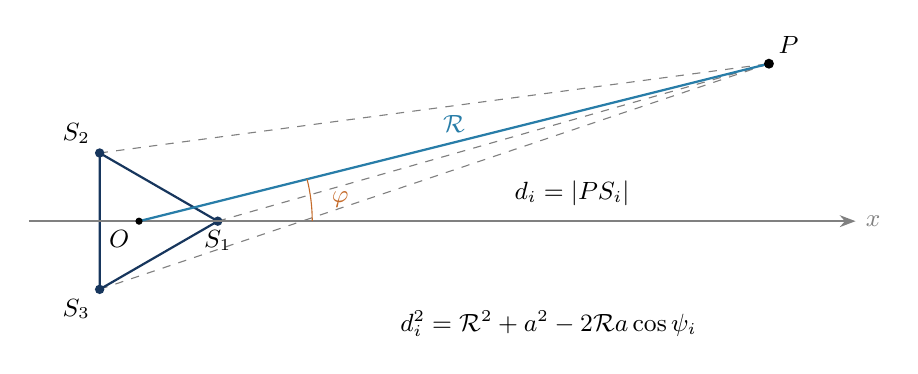
\begin{tikzpicture}
  \coordinate (O) at (0,0);\coordinate (P) at (8.0,2.0);
  \foreach \j/\angle in {1/0,2/120,3/240}{
    \coordinate (S\j) at (\angle:1.0);
    \draw[helper] (S\j)--(P);
    \fill[ink] (S\j) circle (1.7pt);
  }
  \draw[ink,thick] (S1)--(S2)--(S3)--cycle;
  \draw[vec,gray] (-1.4,0)--(9.1,0) node[right] {$x$};
  \draw[thick,field] (O)--(P) node[midway,above] {$\mathcal R$};
  \draw[force] (0:2.2) arc (0:14.0362:2.2) node[midway,right,xshift=4pt] {$\varphi$};
  \fill (O) circle (1.3pt) node[below left] {$O$};
  \fill (P) circle (1.8pt) node[above right] {$P$};
  \node[below] at (S1) {$S_1$};\node[above left] at (S2) {$S_2$};\node[below left] at (S3) {$S_3$};
  \node at (5.5,.35) {$d_i=|PS_i|$};
  \node at (5.2,-1.3) {$d_i^2=\mathcal R^2+a^2-2\mathcal Ra\cos\psi_i$};
\end{tikzpicture}
\begin{tikzpicture}
  \draw[helper] (0,0) circle (2.7);
  \coordinate (G) at (15:2.7);
  \coordinate (Q) at (25:2.7);
  \coordinate (P) at (25:3.35);
  \draw[helper] (0,0)--(P);
  \draw[thick,field] (0,0)--(G) node[midway,below] {$R$};
  \draw[vec,force,line width=1.2pt] (Q)--(P) node[midway,above] {$x$};
  \draw[vec,force] (15:2.7) arc (15:25:2.7) node[midway,left] {$y$};
  \draw[vec,gray] (P)--++(25:1.0) node[right] {$\boldsymbol e_r$};
  \draw[vec,gray] (P)--++(115:1.0) node[above] {$\boldsymbol e_\varphi$};
  \fill (0,0) circle (1.4pt) node[below left] {$O$};
  \fill (G) circle (1.6pt) node[below right] {$P_0$};
  \fill (P) circle (1.6pt) node[below right] {$P$};
  \draw[vec,field] (120:3.0) arc (120:165:3.0) node[midway,left] {$\Omega$};
  \node[anchor=west,align=left] at (5.0,1.6) {$\mathcal R=R+x$，$\varphi=\Omega t+y/R$\\[4pt]$x$：径向微小位移\\[4pt]$y$：切向微小位移\\[4pt]示意图将 $x,y$ 放大显示};
\end{tikzpicture}
\begin{tikzpicture}
  \coordinate (O) at (0,0);\coordinate (S) at (3.6,0);\coordinate (P) at ($(S)+(55:.85)$);
  \draw[helper] (S) circle (.85);
  \draw[thick,ink] (O)--(S) node[midway,below] {$a$};
  \draw[thick,field] (S)--(P) node[midway,left] {$r$};
  \draw[thick,force] (O)--(P) node[midway,above] {$d$};
  \draw[gray] (S)--++(1.3,0);
  \draw[ink] ($(S)+(.4,0)$) arc (0:55:.4) node[midway,right] {$\gamma$};
  \fill (O) circle (1.5pt) node[below left] {$O$};
  \fill[ink] (S) circle (2pt) node[below] {$S_1$};
  \fill (P) circle (1.5pt) node[above right] {$P$};
  \node at (2.8,-1.6) {$d^2=a^2+r^2+2ar\cos\gamma$，$r\ll l$};
\end{tikzpicture}
\end{document}
